%!TEX root = ../Main.tex

\chapter{Tree based methods}

Decision trees are a separate method used for both regression and classification problems. The method works by splitting data into a tree like structure, hence the name of the method. 

When creating a decision tree, we need to divide our feature space into smaller “boxes” in order to create the tree structure. We use an example for explanation:

\begin{figure}[H]
	\centering
	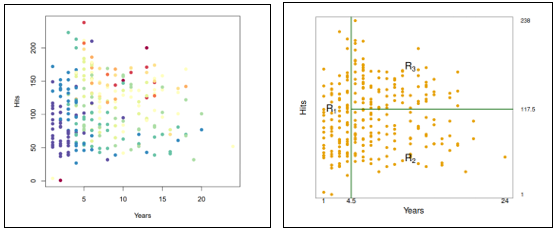
\includegraphics[width=\textwidth]{Img/tree_example.PNG}
	\caption{Example of tree based method for classification}
	\label{fig:tree_example}
\end{figure} 

Here we have baseball salary data, which is depended on years of experience and hits made the previous year. We see from the division that the first internal node comes from 4.5 years of experience. If the player has less than that amount of experience, he will fall into the first segment. If he has more, we have a second division in 117.5 hits. This yields additional two segments as seen from the figure. 

In order to create the segments, we use a method called recursive binary splitting. This is done by starting at the top of the tree for splitting the feature space. It is called a greedy approach because we only consider the current split in each decision, and therefore not taking the reminding part of the tree into consideration when making the splits. Predictions can be made by using the average of all training data points within a region as a measure for that region.  

When creating the trees, me must ensure not to overfit. If we create a very large tree, the regions will be too biased toward the training data. This can be fixed using pruning. If we see that our tree is overfitted with some test data, we can remove one of the leaves from the tree revealing a larger segment. The average of this segment will now have larger residuals towards the training data but perform better with the test data. 

\begin{figure}[H]
	\centering
	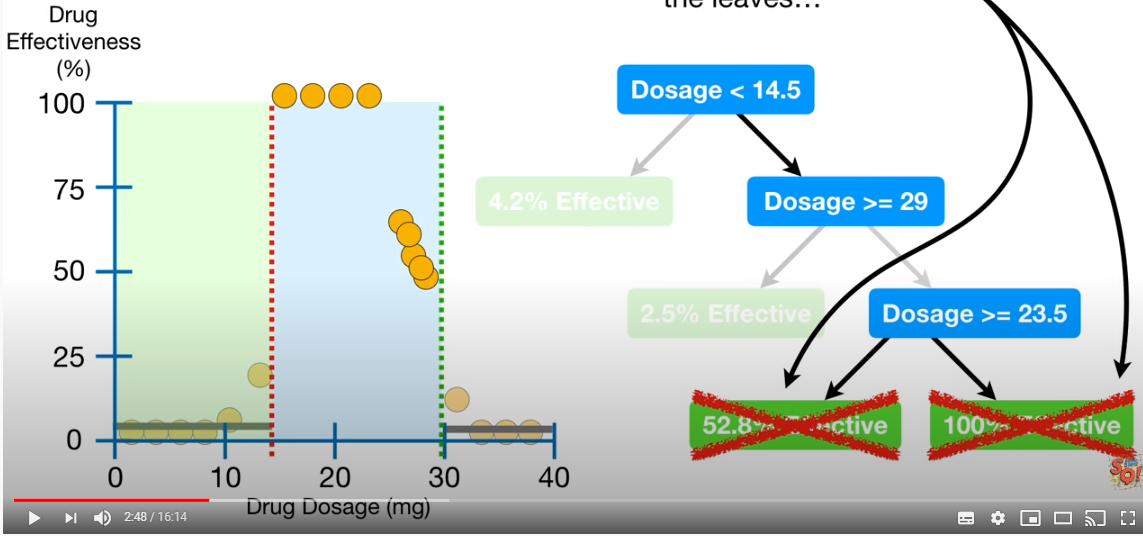
\includegraphics[width=\textwidth]{Img/tree_pruning.PNG}
	\caption{Example of pruning a decision tree}
	\label{fig:tree_pruning}
\end{figure} 

But how do we decide which of the leaves to remove, if pruning is necessary? We start by creating all the trees possible by removing one leaf at the time. Then we create a tree score for each tree which is defined by the following formula:

\begin{equation} \label{eq:3}
Treescore = RSS + \alpha * T 
\end{equation}

RSS is the sum of the residuals squared. This will of course be lowest for the most complex tree, so in order to compensate for that, we add a penalty for complexity. Alpha is a constant found by cross validation and T is the number of terminal nodes on the tree. 

Decision trees are often not as competitive in terms of prediction errors as other methods. However, we have certain things we can do to improve the quality of the tree. One of them is called bootstrap aggregation or bagging. Bagging is a way of reducing the variance of a learning method. It is logical that if we had several different trainings sets available and were able to aggregate our predictions, based on all these training sets, we would be able to get a lower prediction error. However, these training sets are often not available. Therefore, we instead create bootstrap datasets, which as previously described, are subsets drawn from the original set. As we draw these subsets with replacement, we can create different bootstrap sets and use them to average out the result from the datasets.  
 
